\documentclass[twoside]{article}
\input{ISC18-english.sty}
%%%%%%%%%%%%%%%%%%%%%%%%%%%%  Make sure to compile twice for proper cross-references. %%%%%%%%%%%%%%%%%%%%%%%
%%%%%%% For proper display of references, compile the document twice. %%%%%%%%%%%%%%%%%%%%% 
%%%%%%%%%%%%%%% If using TeX Live, compile using pdflatex command %%%%%%%%%%%%%%%%%%%%%%%
\begin{document}
\thispagestyle{empty}
%%%%%%%%%%%%%%%%% Article title header  %%%%%%%%%%%%%%%%%%%%
\fancyhead[LE]{European option valuation}
%%%%%%%%%%%%%%%%% Article authors header   %%%%%%%%%%%%%%%%%%%%
\fancyhead[RO]{P.Yahyavi, N.Modarresi}
\begin{center}
{
\includegraphics [height=25mm, width=150.3mm] {isc18E}} \\
\vspace*{-1.8cm}
%\begin{center}
%\color{blue} 
%{\hspace{0.1cm}\rule{\textwidth}{1mm}}\\
%\end{center}
\vspace*{4cm}
%%%%%%%%%%%%%%%%% Article title  %%%%%%%%%%%%%%%%%%%%
{\Large \bf European option valuation with modified Heston model under stochastic market liquidity}\\
%%%%%%%%%%%%%%%%% Article authors and affiliations %%%%%%%%%%%%%%%%%%%%
{\bf
Parsa Yahyavi$^1$\footnote[2]{{\bf Corresponding Author:} {\tt p\_yahyavi@atu.ac.ir }}, Navide Modarresi$^2$ \\
$^{1,2} $ Department of Mathematics, Allameh Tabataba'i University, Tehran, Iran }
\end{center}
\rule{\textwidth}{0.2mm}\\
%%%%%%%%%%%%%%%%% Article abstract  %%%%%%%%%%%%%%%%%%%%
\noindent{\bf Abstract:}\\
Comprehensive modeling of stock prices plays a critical role in financial derivatives valuation. Although, the classic Heston model captures the stochastic  
volatility, it struggles to replicate the term structure of implied volatility and assumes a perfectly liquid market. To address these inconsistencies, we 
introduce a Heston model by incorporating independent Ornstein–Uhlenbeck processes for both the long‑term mean of volatility and stochastic market 
liquidity. Moreover, we derive an analytical European option pricing formula and validate the model using real market data from leading companies. We 
employ the root mean square error to assess the superiority of the introduced model against three benchmark models in replicating European option prices 
and implied volatility.

\noindent{\bf Keywords:} 
European option pricing, Heston model, Stochastic liquidity, Stochastic volatility \\
\noindent{\bf Mathematics Subject Classification (2020):} $\rm 91G20$, $\rm 91G30$, $\rm 60J76$. \\
\hspace{1cm}\rule{\textwidth}{0.2mm}\\
%%%%%%%%%%%%%%
\section{Introduction}
In 1993, Heston introduced his eponymous model overcorrected the limitations of the Black–Scholes–Merton (BSM) model in capturing 
the implied volatility patterns observed in equity market. The Heston model employs the Cox–Ingersoll–Ross stochastic differential equation (SDE) to cover 
the stochastic volatility. Although the Heston model remedied some limitations of the BSM model, it still produced inaccurate results when replicating 
European option prices and implied volatility.
\cite{He:Chen:2021} extended the Heston model by including the assumption of a stochastic long‑term mean for volatility. They incorporated 
an Ornstein–Uhlenbeck (OU) process to model the long‑term mean of volatility, which in turn led to an improvement in the accuracy of the assessed implied 
volatility term structure. However, they presented their accuracy of the model from the unrealistic assumption of perfect market liquidity.
%
\cite{Amihud:Mendelson:1986} highlighted the effect of liquidity risk on stock prices. \cite{Feng:Hung:Wang:2014} 
represented the stochastic market liquidity framework utilizing an OU process to model market liquidity. Moreover, they employed this methodology for 
European options valuation in \cite{Feng:Hung:Wang:2016}. Following the same assumption, \cite{Cai:Wang:Yu:2024} utilized Lévy processes to 
price vulnerable spread options. \cite{He:Huang:Lin:2025} included credit risk in this framework for more accurate option valuation.  
\cite{Yahyavi:Modarresi:2026} investigated the accuracy of the Heston model for pricing European options, considering the existence 
of jumps in stock prices and the stochasticity of market liquidity.

\noindent
In this paper, we present a modified version of the Heston model that incorporates both a stochastic long-term mean for volatility and the stochasticity of 
market liquidity. To capture these elements, we employ a Cox-Ingersoll-Ross (CIR) model for stochastic volatility, and two OU processes to model the 
stochastic long-term mean and stochastic market liquidity, respectively. Following the approach of \cite{Duffie:Pan:Singleton:2000}, we derive the 
characteristic function of stock price returns. Then, we utilize the relationship between the characteristic function and the Cumulative Distribution Function 
(CDF) to achieve a closed-form formula for European option pricing.

\noindent
Within the empirical analysis, we utilize real market European option price data from famous companies as Apple Inc., Amazon Inc., JPMorgan Chase \& Co., 
and Walmart Inc. to evaluate the performance of proposed model against several benchmarks. As comparative models, we employ the classic Heston model 
which captures only stochastic volatility, the model which accounts only stochastic liquidity, and the model which incorporates both stochastic volatility and a 
stochastic long-term mean. We use the root mean square error (RMSE) to assess the accuracy of each model in replicating observed option prices and implied
volatilities.

\noindent
The remainder of this paper is organized as follows. Section 2 presents the SDEs of the modified Heston model under the risk-neutral measure and the 
corresponding characteristic function. Section 3 includes the derivation of an analytical formula for European option pricing. In Section 4, we report the 
results of the comparison between the proposed model and the benchmark models. Finally, the last section summarizes our findings and concludes the paper.

%%%%%%%%%%%%%%%%%%%%%%%%%%%%%%%%%%%%%%%%%%%%%%%%%%
\section{Modified Heston model}
Let $ \left( \Omega , \mathcal{F} , \left\lbrace \mathcal{F}_t\right\rbrace _{t \geq 0} , \mathbb{Q} \right) $ denote the filtered complete probability space, 
where $ \mathbb{Q} $ is the risk-neutral measure and it is endowed with the filtration $ \left\lbrace \mathcal{F}_t\right\rbrace _{t \geq 0} $ where $t \in 
\left[ 0 , T \right] $ for a fixed expiration time $ T $. We define the model dynamics with respect to measure $ \mathbb{Q} $ as below.
%
\begin{equation}
\label{St under P with at and vt}
\left\{
\begin{array}{l}
\frac{dS_t}{S_{t}} = r dt +  \sqrt{\nu_t} dB_{1,t} + \beta a_t  dB_{2,t}, \\[5pt]
d\nu_t = \kappa (\theta_t - \nu_t) dt + \sigma_1 \sqrt{\nu_t} dB_{3,t}, \\[5pt]
d\theta_t = \alpha dt + \sigma_2  dB_{4,t}, \\[5pt]
da_t = \kappa_a (\theta_a - a_t) dt + \sigma _{3}  dB_{5,t}, 
\end{array}
\right.
\end{equation}
%
where $ r $ is the risk-free rate of return, $ \nu_t $ is the stochastic volatility, $ \kappa $ is mean reversion speed, $ \theta_t $ is the stochastic mean level 
of volatility, $ \sigma_1 $ is volatility of volatility, $ \alpha $ is the drift of mean level of volatility, $ \sigma_2 $ is the volatility of mean level of volatility, 
$ a_t $ is stochastic market liquidity, $ \kappa^a $ is mean reversion speed of market liquidity, $ \theta^a $ is mean level of market liquidity and 
$ \sigma_3 $ is volatility of market liquidity. All Brownian motion processes are mutually independent under measure $ \mathbb{Q} $ except $ B_{1,t} $ 
and $ B_{3,t} $ with correlation $ \rho $ and $ B_{2,t} $ and $ B_{5,t} $ with correlation $ \rho_a $. 
%
\begin{rem}\label{rm1}
If $ \beta=\alpha=\sigma_2=\kappa_a=\theta_a=\sigma _{3}=0 $ , the proposed model reduces to the Heston model. 
If $ \alpha=\sigma_2=\kappa=\sigma _{1}=0 $ , the proposed model reduces to the \cite{Feng:Hung:Wang:2014} model. And, if 
$ \beta=\kappa_a=\theta_a=\sigma _{3}=0=0 $ , the proposed model reduces to the \cite{He:Chen:2021} model.
\end{rem}
%
\noindent
By assuming $X_t := \ln(S_t)$, we derive the characteristic function of $X_t$ employing the methodology presented by \cite{Duffie:Pan:Singleton:2000} 
for affine jump-diffusion models. The exponential-affine representation of the characteristic function is presented in the following theorem. 
%
\begin{thm}\label{theorem_Xt}
Let the underlying stock price follow the model specified in (\ref{St under P with at and vt}), then, the characteristic function of $X_t = \ln(S_t)$ is given by
\begin{equation}\label{AffineChf}
\phi(u,t,T;x,\nu, a, \theta) = \exp \left\lbrace A(u;\tau) + B(u;\tau)a + C(u;\tau)a^2 +D(u ;\tau)\nu + E(u ;\tau)\theta + iux \right\rbrace , 
\end{equation}
where $i=\sqrt{-1}$, $\tau=T-t$, $ T $ is the maturity time of the European option, and the coefficient functions are
%
\begin{align*}
A &= \frac{1}{4} \left( \left( a_1 - 2(i \sigma_3 \beta \rho_{a} u - \kappa_a) \right) \tau 
- 2 \ln\left( \frac{1 - b_1 e^{a_1 \tau}}{1 - b_1} \right) \right) 
\nonumber \\ &\quad 
+ \int_0^\tau \left( \frac{1}{2} \sigma_3^2 B^2(u; s) + \kappa_a \theta_a B(u; s) + \frac{1}{2} \sigma_2^2 E^2(u; s) 
+ \alpha E(u; s)  \right) ds + r i u \tau,  %\label{eq:A} 
\\
B &= -\frac{ \kappa_a \theta_a \left( a_1 - 2(i \sigma_3 \beta \rho_a u - \kappa_a) \right)}{a_1 \sigma_3^2}
\frac{\left( 1 - e^{\frac{1}{2} a_1 \tau} \right)^2}{1 - b_1 e^{a_1 \tau}},  %\label{eq:B} 
\\
C &= \frac{a_1 - 2(i \sigma_3 \beta \rho_a u - \kappa_a)}{4 \sigma_3^2} \frac{1 - e^{a_1 \tau}}{1 - b_1 e^{a_1 \tau}},  %\label{eq:C}
\\
D &= \frac{a_2 - (i \sigma_1 \rho u - \kappa) }{\sigma_1^2} \frac{1 - e^{a_2 \tau}}{1 - b_2 e^{a_2 \tau}},  %\label{eq:D}
\\
E &= \frac{\kappa}{\sigma^2_1}\left[ \left( a_2 - (i \sigma_1 \rho u - \kappa )  \right)\tau  
+ 2 ln\left( \frac{1-b_2e^{a_2\tau}}{1-b_2} \right)  \right],  %\label{eq:E}
\end{align*}
and
\begin{align*}
a_1 &= 2\sqrt{( i \sigma_3 \beta \rho_a  u - \kappa_a )^2 + \sigma_3^2 \beta^2 (i u + u^2)}, \\
a_2 &= \sqrt{(i \sigma_1   \rho  u -  \kappa )^2 + \sigma_1^2 (i u + u^2)}, \\
b_1 &= \frac{2( i \sigma_3 \beta \rho_a  u - \kappa_a) - a_1}{2(i \sigma_3 \beta \rho_a  u - \kappa_a) + a_1}, \\
b_2 &= \frac{(i \sigma_1   \rho  u -  \kappa ) - a_2}{(i \sigma_1   \rho  u -  \kappa) + a_2},
\end{align*}
\end{thm}
\noindent
where all parameters are defined in the model represented in (\ref{St under P with at and vt}). In the following section, we employ the characteristic 
function represented in Theorem \ref{theorem_Xt} to derive an analytic formula for European option valuation.

%%%%%%%%%%%%%%%%%%%%%%%%%%%%%%%%%%%%%%%%%%%%%%
\section{European option price formula}
To derive the European option price, we utilize the relation between the characteristic function and the CDF in the following theorem.
%
\begin{thm}\label{theorem_relation}
Given an arbitrary random variable $ X $ with Lebesgue integrable density function $ f $ and characteristic function $ \phi $, if the mean of $ X $ exists
then the following relation holds between characteristic function $ \phi $ and $ F $ as the CDF of $ X $
\begin{equation}\label{RealtionPhiandF}
F\left( x\right) =\frac{1}{2} - \frac{1}{2\pi}\int^{\infty}_{0} \Delta \left[ \frac{\phi\left( u \right) e^{-iux}}{iu} \right] du,
\end{equation}
where $ \Delta g(u)=g(u)+g(-u) $.
\end{thm}
\noindent
By following the risk-neutral pricing methodology, the price of an European call option with strike price $K$, maturity $T$, and underlying stock $S_t$ is 
formulated as follows.
\begin{equation}\label{OptionPrice}
C(S_t, K, \tau, \nu_t, a_t)=e^{-r\tau} \mathbb{E}^{\mathbb{Q}}\left[ (S_T - K )^{+} \vert {\mathcal{F}_t}^{agg} \right], 
\end{equation}
where $ \tau=T-t $ and $ {\mathcal{F}_t}^{agg} =\left\lbrace  {\mathcal{F}_t}^{B_{1,t}}  \vee  {\mathcal{F}_t}^{B_{2,t}}  \vee
{\mathcal{F}_t}^{B_{3,t}} \vee {\mathcal{F}_t}^{B_{4,t}}  \vee {\mathcal{F}_t}^{B_{5,t}}    \right\rbrace_{t \geq 0}$. 
We are able to redefine the European option price by employing the relation \eqref{RealtionPhiandF} in Equation \eqref{OptionPrice} as below.
%
\begin{equation}\label{Risk-neutral option price} 
C(I_1,I_2,\tau) = e^{-r\tau} \left[ I_1 - K I_2 \right],
\end{equation}
where 
\begin{align*}
I_1 &= \phi(-i,t,T;x,\nu, a, \theta) \left[ \frac{1}{2} + \frac{1}{\pi} \int_0^{\infty} \mathrm{Re} \left( \frac{ e^{-iu \ln(K)} }{iu} 
\frac{\phi(u - i,t,T;x,\nu,a, \theta)}{\phi(-i,t,T;x,\nu,a, \theta)} \right) du \right], %\label{Integ1_solved} 
\\
I_2 &= \frac{1}{2} + \frac{1}{\pi} \int_0^{\infty} \mathrm{Re} \left( \frac{ e^{-iu \ln(K)} }{iu} \phi(u,t,T;x,\nu,a, \theta) \right) du, 
%\label{Integ2_solved}
\end{align*}
and $ \phi(u,t,T;x,\nu,\alpha,\theta) $ is the characteristic function derived in Theorem \ref{theorem_Xt}. In the following section, we employ the analytic 
formula in (\ref{Risk-neutral option price}) to compare the accuracy of the proposed model in replicating real market European option prices and implied 
volatility against benchmarks.

%%%%%%%%%%%%%%%%%%%%%%%%%%%%%%%%%%%%%%%%%%%%%%%%%%%%%%
\section{Model's accuracy comparison}
We utilize real market data from European option chains for four distinct stocks, Apple Inc., Amazon Inc., JPMorgan Chase \& Co., and Walmart Inc. We also 
employ the RMSE function to compare the efficiency of the represented model against benchmarks. The features captured by each 
benchmark model are briefly discussed in Table \ref{tab1}.
%
\vspace{-0.3cm}
\begin{table}[h!]
\begin{center}
\small
\caption{Benchmark models discussion.}\label{tab1}
\begin{tabular}{|c|ccc|}
  \hline
  Model & Stochastic volatility & Stochastic liquidity & Stochastic long-term mean \\  \hline \hline
  Heston    & $ \checkmark $ & $\times$ & $\times$ \\
  Feng       & $\times$                       & $ \checkmark $ & $\times$ \\
  HeChan  & $ \checkmark $  & $\times$ &  $ \checkmark $ \\  
  Ours       & $ \checkmark $  & $ \checkmark $ &  $ \checkmark $ \\ \hline
\end{tabular}
\end{center}
\end{table}
%
As illustrated in Figures \ref{fig1} and \ref{fig2}, the proposed model exhibits the lowest RMSE values when compared with benchmark models in replicating 
European option prices and implied volatility, respectively.
The proposed model demonstrates enhanced accuracy in replicating the prices of European option chains, even when the chain is dense with multiple strike 
prices, as shown in Panel a) of Figure \ref{fig1}. Furthermore, as observed in Figure \ref{fig2}, the introduced model effectively captures the volatility smile 
curve, particularly in the at-the-money region.
\vspace{-0.1cm}
\begin{figure}[h!]
\begin{center}
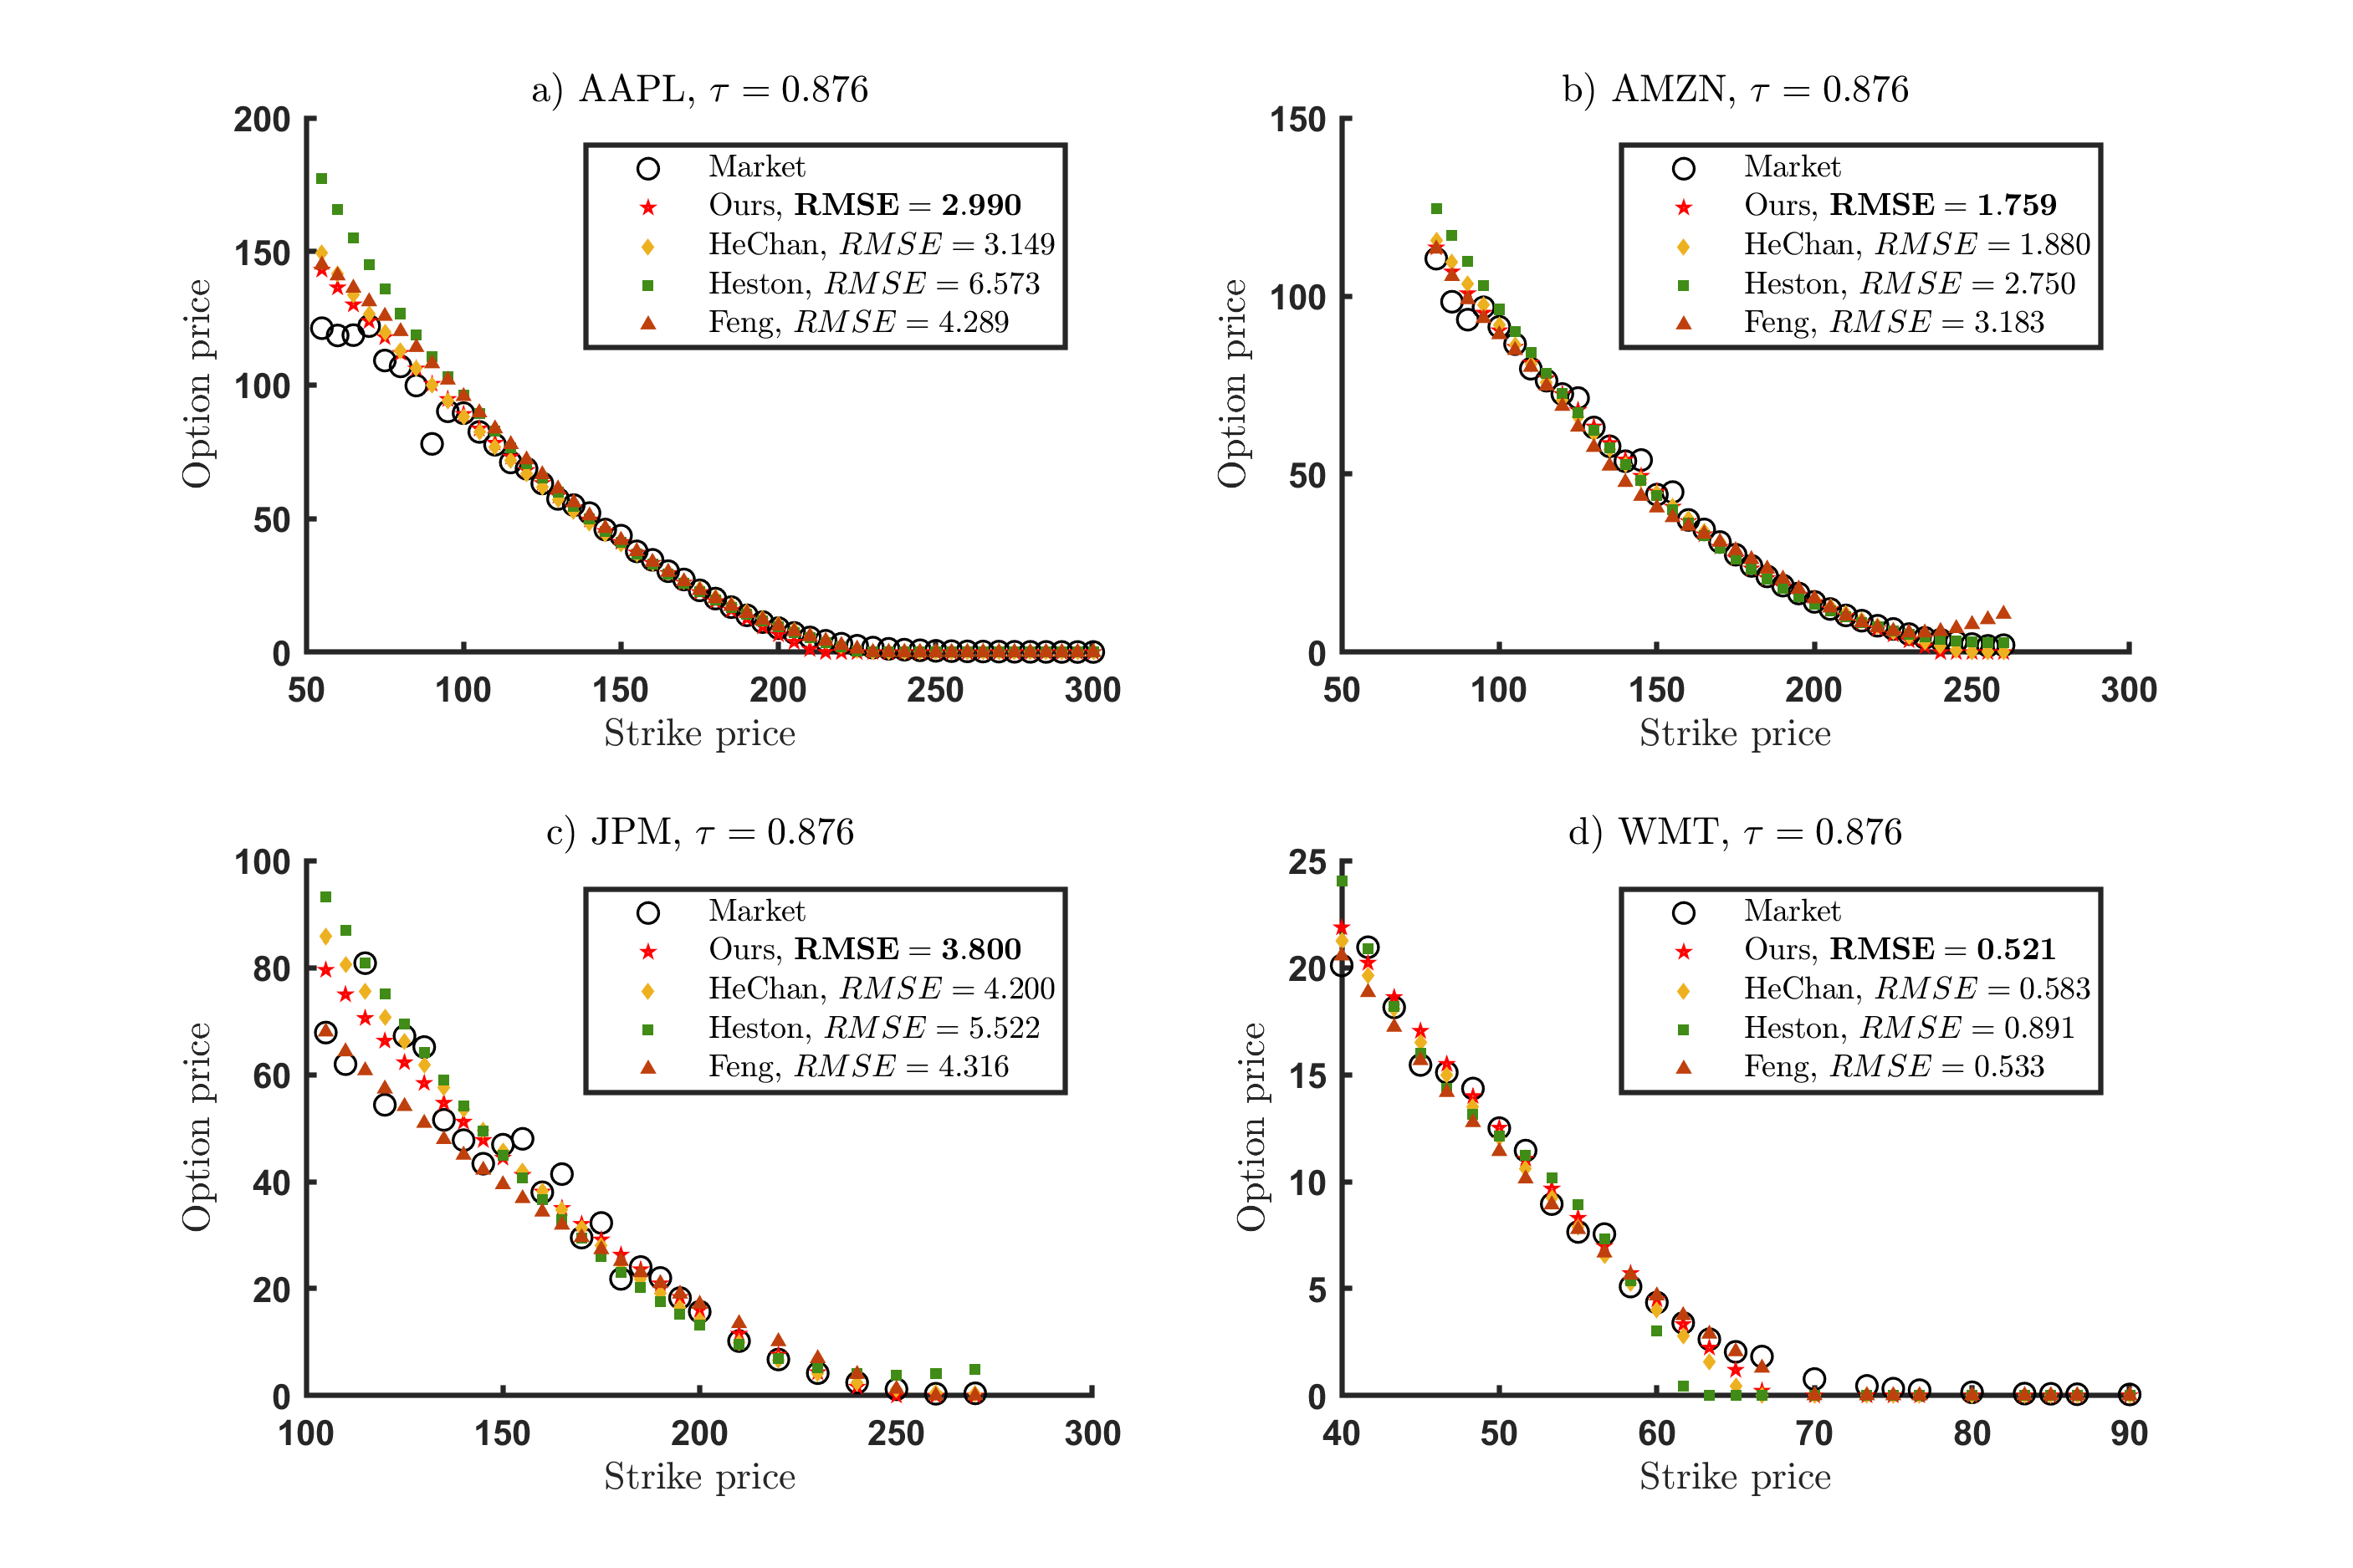
\includegraphics[width=\textwidth]{figure_combined_compact}
\vspace{-1.4cm}
\caption{\footnotesize{Comparison of the proposed model's replication of European option prices against benchmarks.}}\label{fig1}
\end{center}
\end{figure}
%
\begin{figure}[h!]
\begin{center}
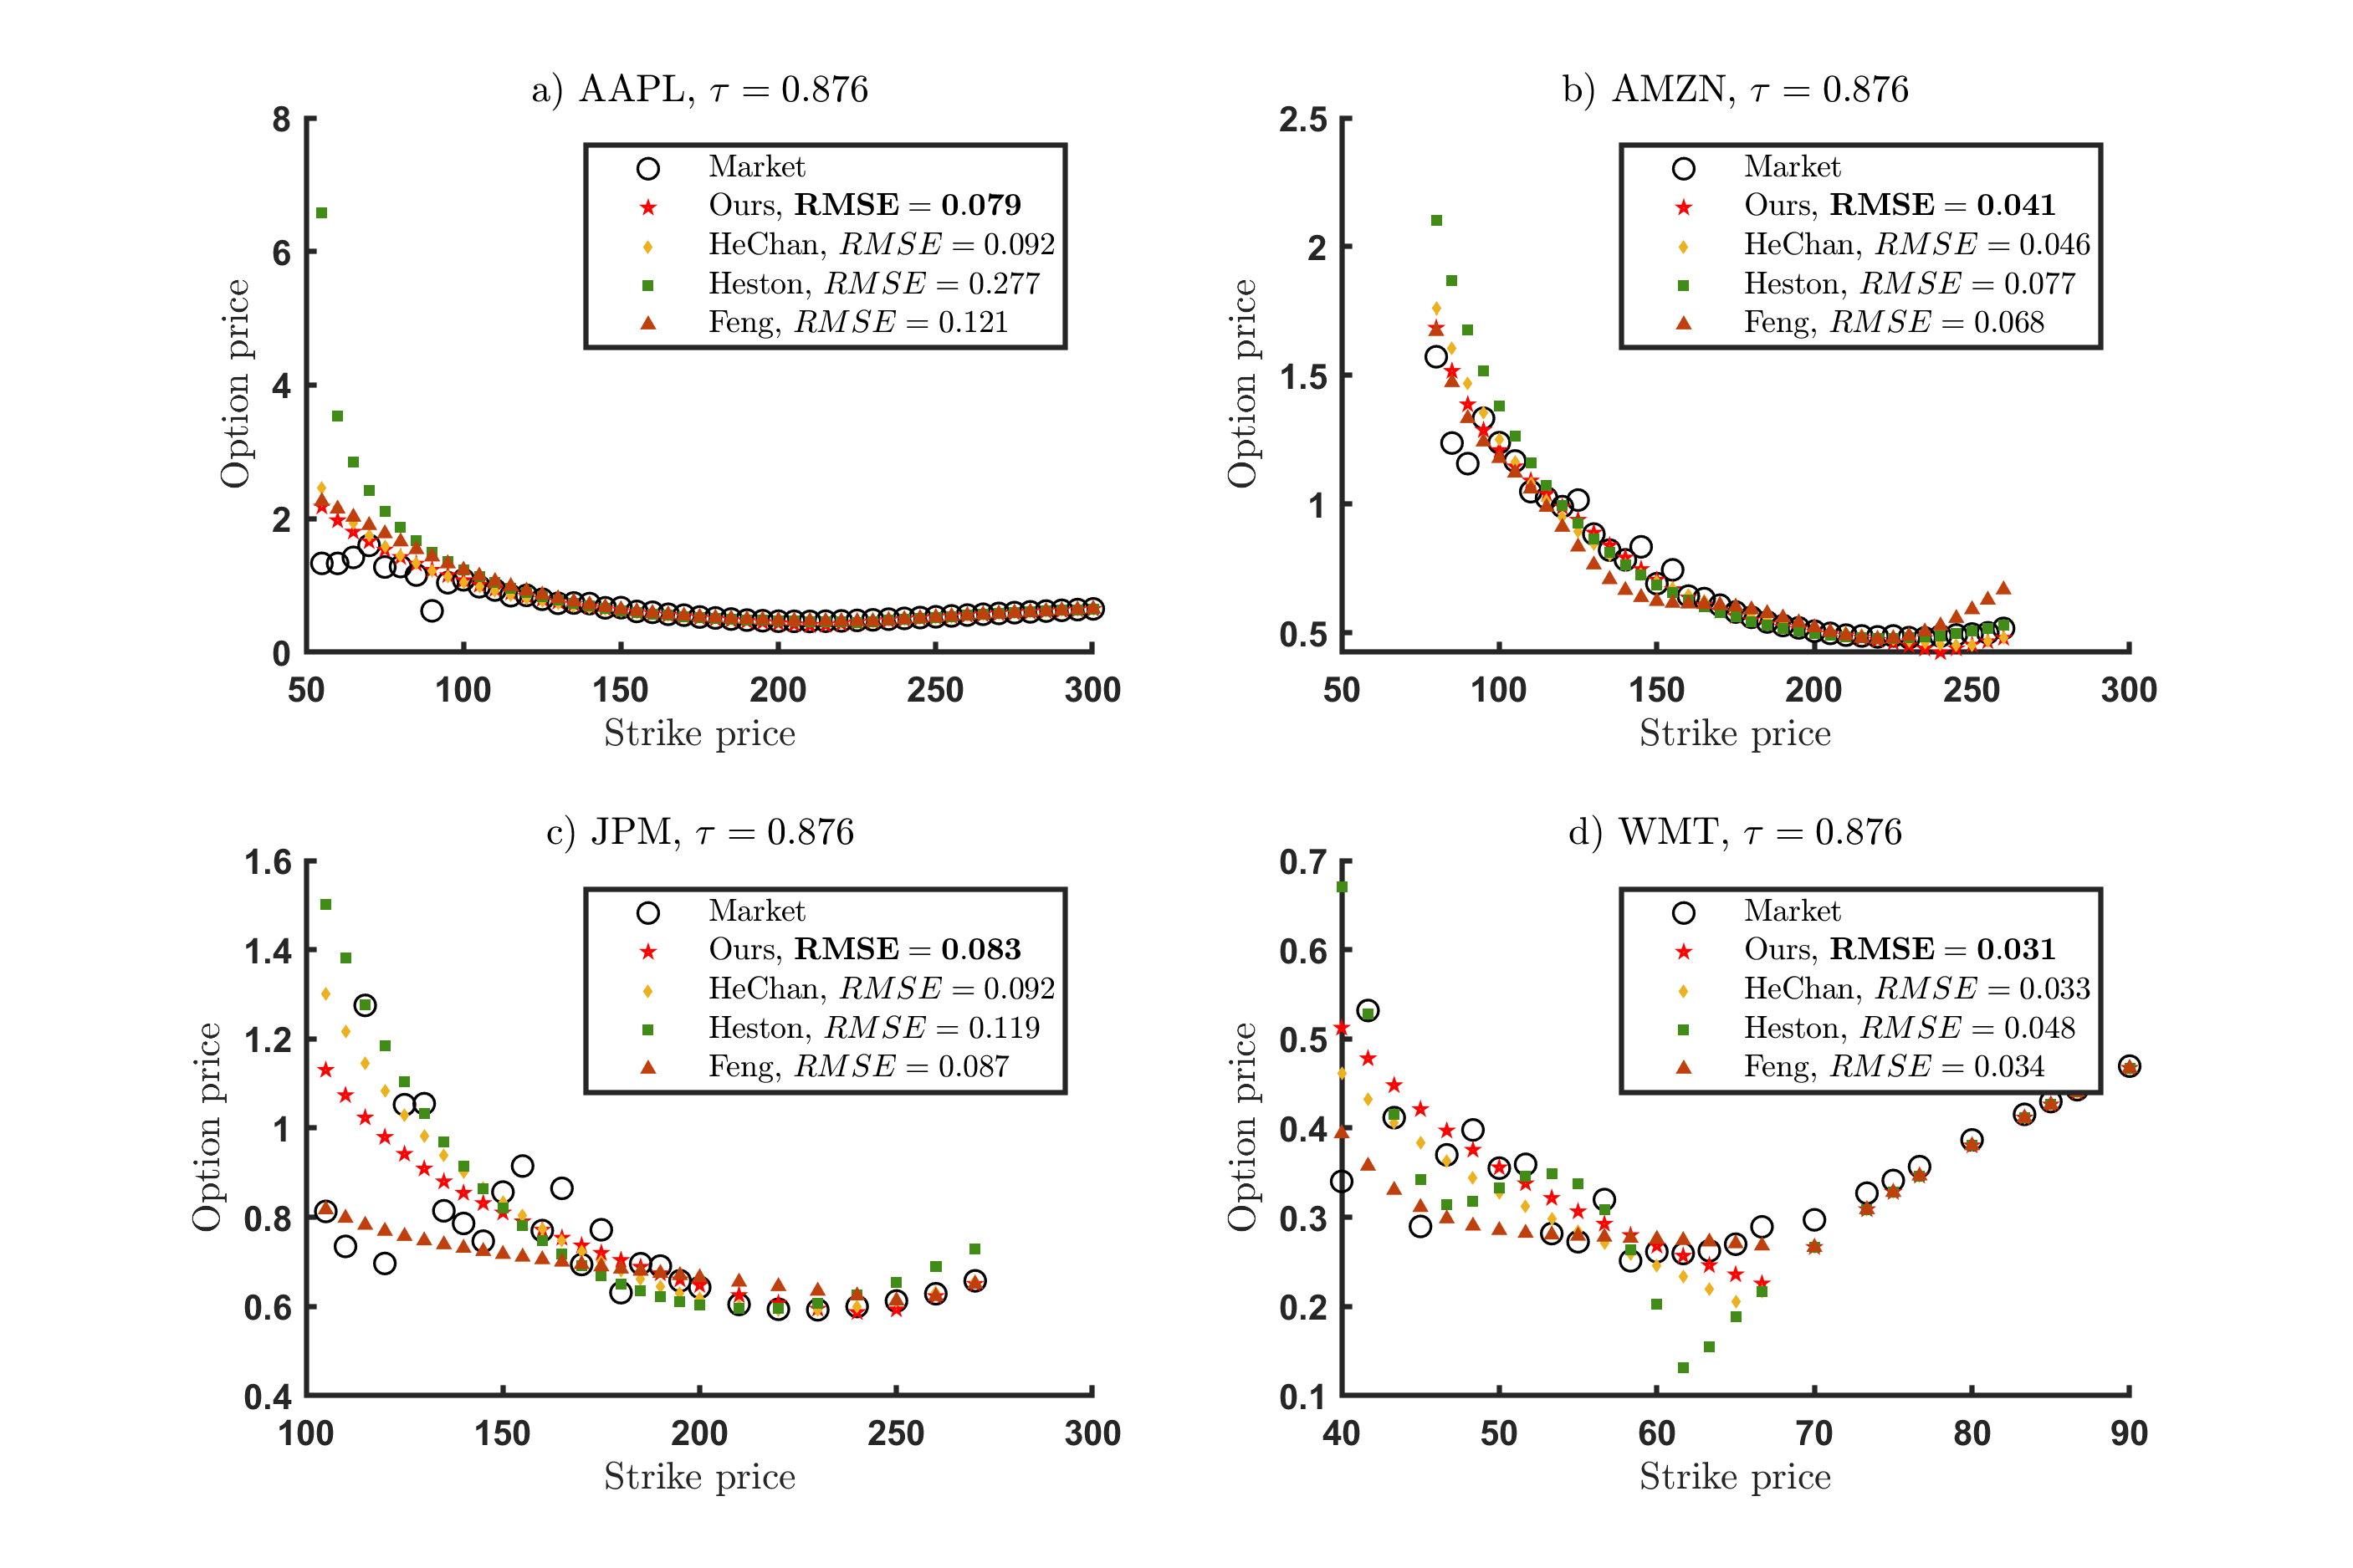
\includegraphics[width=\textwidth]{figure_combined_compact_IV}
\vspace{-1.4cm}
\caption{\footnotesize{Comparison of the proposed model's replication of implied volatility against benchmarks.}}\label{fig2}
\end{center}
\end{figure}

%%%%%%%%%%%%%%%%%%%%%%%%%%%%%%%%%%%%%%%%%%%%%%%%%%%%%%%%
\section*{Discussion and Conclusion} 
In this paper we have introduced a comprehensive model for pricing European options, integrating stochastic volatility, long-term mean of volatility, and 
market liquidity simultaneously. Furthermore, we have utilized real market data to perform a comparison between the introduced model and benchmarks. 
The empirical analysis results demonstrate the superiority of proposed model in achieving the lowest RMSE values. 

%%%%%%%%%%%%%%%%%%%%%%%% References %%%%%%%%%%%%%%%%%%%%%%%%%%%%%

\begin{thebibliography}{9}

\bibitem[Amihud and Mendelson (1986)]{Amihud:Mendelson:1986}
Amihud, Y. and Mendelson, H. (1986), Liquidity and stock returns, {\it Financial Analysts Journal}, 42, 43-48.

\bibitem[Cai et al. (2024)]{Cai:Wang:Yu:2024}
Cai, C. and Wang, X. and Yu, B. (2024), Pricing vulnerable spread options with liquidity risk under Lévy processes, 
{\it The North American Journal of Economics and Finance}, 72, 102-124.

\bibitem[Duffie et al. (2000)]{Duffie:Pan:Singleton:2000}
Duffie, D. and Pan, J. and Singleton, K. (2000), Transform Analysis and Asset Pricing for Affine Jump-Diffusions, 
{\it Econometrica}, 68, 1343-1376.

\bibitem[Feng et al. (2014)]{Feng:Hung:Wang:2014}
Feng, S. P. and Hung, M. W. and Wang, Y. H. (2014), Option pricing with stochastic liquidity risk: Theory and evidence,
{\it Journal of Financial Markets}, 18, 77-95.
 
\bibitem[Feng et al. (2016)]{Feng:Hung:Wang:2016}
Feng, S. P. and Hung, M. W. and Wang, Y. H. (2016), The importance of stock liquidity on option pricing,
{\it International Review of Economics \& Finance}, 43, 457-467.

\bibitem[He and Chen (2021)]{He:Chen:2021}
He X. and Chen W. (2021), A closed-form pricing formula for European options under a new stochastic volatility model with a stochastic long-term mean, 
{\it Math. Financ. Econ.} 15, 381–396.

\bibitem[He et al. (2025)]{He:Huang:Lin:2025}
He, X. J. and Huang, S. D. and Lin, S. (2025), A closed-form solution for pricing European-style options under the Heston model with credit and liquidity risks,
{\it Communications in Nonlinear Science and Numerical Simulation}, 143. 

\bibitem[Yahyavi and Modarresi (2026)]{Yahyavi:Modarresi:2026}
Yahyavi, P. and Modarresi, M. (2026), A Heston model with jumps and stochastic liquidity risk in European option pricing, 
{\it Review of Derivatives Research}, Accepted manuscript. 


\end{thebibliography}
 \end{document}

